\documentclass{article}


\usepackage{graphicx} % for including graphics
\graphicspath{{images/}}
\usepackage{amsmath}  % for advanced math formatting
\usepackage{hyperref}  % for hyperlinks
\usepackage{appendix}
\usepackage[table]{xcolor}
\usepackage{caption}
\usepackage{enumitem}
\usepackage{amsmath}
\usepackage{siunitx}
\usepackage{wrapfig}
\usepackage{float}
\usepackage{subcaption}




\begin{document}

\title{Lesstof tentamen HARONT}
\author{Michel Vollmuller}
\date{\today}

\maketitle


\tableofcontents

\newpage

\section{Hoogfrequent}

    \subsection{les 1 Elektromagnetische golven}
    Date : 1 december 2023

\subsubsection{Overdracht}

Een elektromagnetische golf plant zich voor in vacuüm(ether) met de
lichtsnelheid.
In een kabel (koper/optisch) plant de golf zich met een lagere snelheid voort
dan de lichtsnelheid.
\begin{itemize}[label=$\bullet$]
    \item Een EM golf bestaat uit een elektrisch en magnetisch veld.
    \item Het elektrische en magnetische veld staan loodrecht ten opzichte van elkaar.
    \item De richting van het elektrische veld wordt    de polarisatierichting genoemd.
    \item labda = c/f
  \end{itemize}

\begin{figure}[H]
\centering
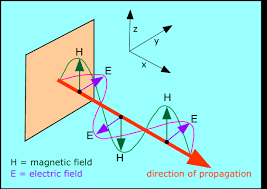
\includegraphics[scale=0.8]{EM signaal.png}
\caption{EM Signaal.}
\end{figure}

\begin{figure}[H]
\centering
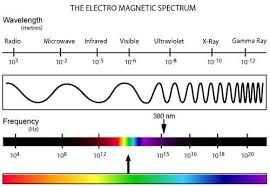
\includegraphics[scale=0.8]{elektromagnetisch spectrum.jpeg}
\caption{Elektromagnetisch spectrum}
\end{figure}


\subsubsection{Golflengte}

Voortplantingssnelheid in de vrije ruimte, wordt lichtsnelheid ‘c’
genoemd en is 3.108 m/s. 
Het verband tussen de golflengte en de frequentie: labda = c/f

\begin{figure}[H]
\centering
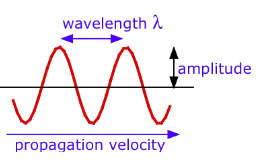
\includegraphics[scale=0.8]{Golflengte.png}
\caption{Golflengte}
\end{figure}

\subsubsection{Verkortingsfactor}

De voorplantingssnelheid in een medium. Dus bijvoorbeeld een kabel
of fiber is lager.\\
in vacuum geldt \(c = \sqrt{\frac{1}{\varepsilon_0 \mu_0}}\)\\
waarin \(\varepsilon_0\) de elektische veldconstante is\\
waarin \(\mu_0\) de magnetische veldconstante is\\

In een kabel zijn deze constanten hoger waardoor de snelheid lager wordt. Deze verlaging wordt de Verkortingsfactor genoemd. De Verkortingsfactor van bijvoorbeeld een coaxkabel is 2/3.\\

Een Verkortingsfactor heeft  gevolgen voor de golflengte in de kabel! Je moet hier bij de volgende zaken rekening mee houden:
\begin{itemize}[label=$\bullet$]
    \item Board design, lengte van printsporen
    \item Antenne-afmetingen
    \item Lichtbreking (fiber communication)
\end{itemize}

\subsubsection{Impedantie}

De impedantie (\(Z\)) wordt gegeven door de som van de reële component (\(R\)), ook wel de weerstand genoemd, en de imaginaire component (\(jX\)), ook wel reactantie genoemd. Deze reactantie kan inductief of capacitief zijn.

\[
Z = R + jX
\]

Waarbij:
\begin{align*}
R & : \text{Reële component (weerstand)} \\
jX & : \text{Imaginaire component (reactantie)}
\end{align*}

De karakteristieke impedantie (\(Z_0\)) van een kabel of vierpool is de impedantie die aan de ingang gelijk wordt aan de impedantie waarmee je de uitgang afsluit. Wanneer je hieraan voldoet, heb je op alle punten de juiste aanpassing en dus optimale vermogensoverdracht!

\[
Z_0
\]

Zkar van een kabel: \\
Een klein stukje kabel is voor te stellen als een vierpool:
\begin{figure}[H]
\centering
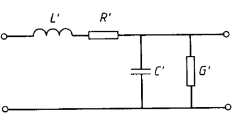
\includegraphics[scale=0.8]{vierpool.png}
\caption{Vierpool}
\end{figure}
Voor een verliesvrije kabel geldt R=0 en G=oneindig
\[
Zkar = \sqrt{L / C}
\]

\subsubsection{Afsluiten van transmissielijnen}

We willen een maximale vermogensoverdracht van een bron naar een belasting bereiken wanneer de impedantie van de bron (\(Z_i\)) gelijk is aan de impedantie van de belasting (\(Z_l\)). Wanneer dit niet het geval is, treedt bij hoogfrequente signalen reflectie op.

Deze situatie heeft twee ongewenste gevolgen:
\begin{enumerate}
  \item Vermogensverlies
  \item Mogelijke beschadiging van de zender (eindtrap) door extra dissipatie van gereflecteerd vermogen. Dit kan leiden tot oververhitting. Meer geavanceerde systemen zijn vaak beschermd tegen dergelijke situaties.
\end{enumerate}

karakteristiek korgesloten = Alle energie komt terug. De spanning wordt gereflecteerd in tegenfase.
\begin{figure}[H]
\centering
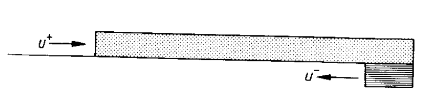
\includegraphics[scale=0.8]{karakteristiek kortgesloten.png}
\caption{karakteristiek kortgesloten}
\end{figure}

karakteristiek open = Alle energie komt terug. De spanning wordt gereflecteerd in fase.
\begin{figure}[H]
\centering
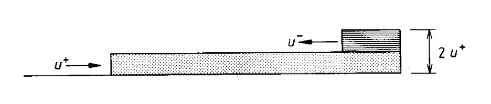
\includegraphics[scale=0.8]{karakteristiek open.png}
\caption{karakteristiek open}
\end{figure}

\subsubsection{Pulsechometing}

Pulseecho-metingen of een Optical Time Domain Reflectometer (OTDR) worden gebruikt bij glasvezelkabels. Op de positie van de breuk bevindt zich in feite een open uiteinde (de energie komt terug!). Door de tijd te meten tussen de verstuurde en gereflecteerde puls is de positie van de breuk vast te stellen! De essentiële parameter van een kabel die hiervoor nodig is, is de verkortingsfactor; deze bepaalt de snelheid van de elektromagnetische golf in de kabel (\(c\)).

\subsubsection{decibel}
\begin{figure}[H]
\centering
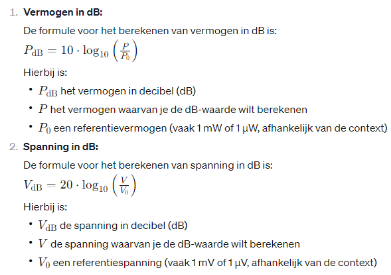
\includegraphics[scale=1.1]{vermogen.png}
\end{figure}

\begin{itemize}
    \item Wat is dBm? 
    \[ \text{dBm} = 10 \cdot \log_{10}\left(\frac{P}{1 \, \text{mW}}\right) \]
  
    \item Wat is dBi? 
    \begin{itemize}
      \item Decibels ten opzichte van een isotrope straler.
      \item Isotrope straler? (Komen we nog op terug)
    \end{itemize}
  
    \item En dBd? 
    \begin{itemize}
      \item Decibels ten opzichte van een dipool. (Komen we ook nog op terug)
    \end{itemize}
  \end{itemize}


    \newpage
    \subsection{les 2 Analoge modulatie}
    Date : 8 december 2023

\subsubsection{Moduleren}
Het aanbrengen van informatie in een draaggolf wordt vaak gemodelleerd als:

\[ U_c(t) = \hat{U}_c \cdot \cos(2\pi f_c t + \alpha) \]

waarbij:
\begin{itemize}
  \item \(U_c(t)\) de gemoduleerde draaggolf is,
  \item \(\hat{U}_c\) de amplitude van de draaggolf,
  \item \(f_c\) de frequentie van de draaggolf,
  \item \(\alpha\) de fasehoek.
\end{itemize}

Amplitude Modulatie (AM) houdt in dat de amplitude \(\hat{U}_c\) wordt gevarieerd.

Frequentiemodulatie (FM) houdt in dat de frequentie \(f_c\) wordt gevarieerd.

Phasemodulatie (PM) houdt in dat de fasehoek \(\alpha\) wordt gevarieerd.

\begin{figure}[H]
\centering
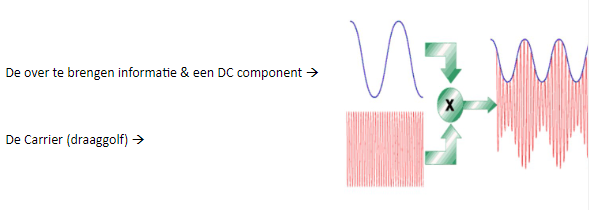
\includegraphics[scale=0.8]{AM.png}
\caption{Amplitude Modulatie}
\end{figure}

Modulatiediepte (\(m\)) geeft aan hoe sterk er gemoduleerd wordt en wordt bepaald door:

\[ m = \frac{\hat{U}_m}{\hat{U}_c} \times 100\% \]

waarbij:
\begin{itemize}
  \item \(m\) de modulatiediepte is,
  \item \(\hat{U}_m\) de amplitude van het informatiesignaal is,
  \item \(\hat{U}_c\) de amplitude van het carriersignaal is.
\end{itemize}

In het frequentiespectrum ontstaan drie frequentiecomponenten (wanneer het informatiesignaal uit slechts één frequentie bestaat):

\begin{enumerate}
  \item De carrierfrequentie \(f_c\)
  \item Zijband 1: \(f_c + f_m\)
  \item Zijband 2: \(f_c - f_m\)
\end{enumerate}

waarbij:
\begin{itemize}
  \item \(f_c\) de draaggolf frequentie is,
  \item \(f_m\) de frequentie van het informatiesignaal is.
\end{itemize}

\begin{figure}[H]
\centering
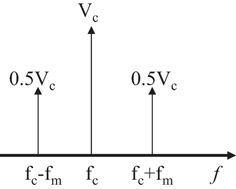
\includegraphics[scale=0.8]{frequentiespectrum AM.png}
\caption{Frequent AM}
\end{figure}

Het vermogensspectrum is als volgt te bepalen:

\begin{itemize}
  \item Voor de Carrier geldt:
  \[ P_c = \left(\frac{\hat{U}_c}{\sqrt{2}}\right)^2 \div R_{\text{load}} \, \text{(Watt)} \]

  \item Voor elke van de zijbanden geldt:
  \[ P_{zb} = \left(\frac{m\hat{U}_c}{2\sqrt{2}}\right)^2 \div R_{\text{load}} = \frac{m^2}{4} \cdot \left(\frac{\hat{U}_c}{\sqrt{2}}\right)^2 = \frac{P_c \cdot m^2}{4} \]
\end{itemize}

waarbij:
\begin{itemize}
  \item \(P_c\) het vermogen van de carrier is,
  \item \(P_{zb}\) het vermogen van elke zijband is,
  \item \(\hat{U}_c\) de amplitude van het carriersignaal is,
  \item \(m\) de modulatiediepte is,
  \item \(R_{\text{load}}\) de belastingsweerstand is.
\end{itemize}

\vspace{0.5cm}
Wat zijn de voordelen van AM?
\begin{itemize}
  \item Eenvoudige demodulatie.
  \item De carrier is altijd aanwezig en afstembaar.
\end{itemize}

Wat zijn de nadelen van AM?
\begin{itemize}
  \item Storingsgevoeligheid (amplitude).
  \item Relatief veel vermogen waarin geen informatie zit.
\end{itemize}

\subsubsection{Single Side Band (SSB)}
Single Side Band (SSB) is een modulatietechniek die wordt gebruikt in communicatiesystemen. In SSB wordt slechts één zijband van het gemoduleerde signaal overgedragen, samen met de draaggolf, in plaats van beide zijbanden zoals bij Amplitude Modulatie (AM).

De wiskundige representatie van een SSB-signaal is als volgt:

\[ U(t) = A_c \cdot m(t) \cdot \cos(2\pi f_c t) \]

waarbij:
\begin{itemize}
  \item \(U(t)\) is het SSB-signaal,
  \item \(A_c\) is de amplitude van de draaggolf,
  \item \(m(t)\) is het informatiesignaal,
  \item \(f_c\) is de frequentie van de draaggolf.
\end{itemize}

\begin{figure}[H]
\centering
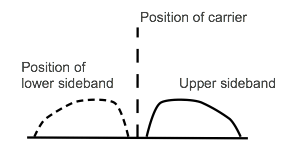
\includegraphics[scale=0.8]{single-sideband-ssb-overview.png}
\caption{single side band overview}
\end{figure}

De voordelen van SSB zijn onder andere een efficiënter gebruik van het radiospectrum en verminderde vermogensvereisten. Echter, demodulatie van SSB vereist complexere apparatuur in vergelijking met AM.

\subsubsection{Frequentie Modulatie (FM)}
FM is een goed alternatief voor AM.

Voordelen:
\begin{itemize}
  \item Minder storingsgevoelig, informatie zit niet in de amplitude.
  \item Constant vermogen.
\end{itemize}

Nadelen:
\begin{itemize}
  \item Grotere bandbreedte.
  \item Complexere hardware.
\end{itemize}

\begin{figure}[H]
\centering
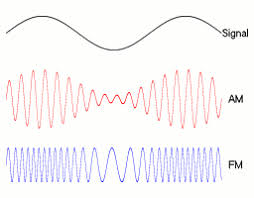
\includegraphics[scale=0.8]{FM.jpeg}
\caption{FM vs AM}
\end{figure}
    

    \newpage
    \subsection{les 3 Digitale modulatie}
    Date : 14 december 2023

\subsubsection{Amplitude Shift Keying 'ASK'}

Voordelen:
\begin{itemize}
  \item Eenvoudig en goedkoop.
  \item Weinig bandbreedte nodig.
\end{itemize}

Nadelen:
\begin{itemize}
  \item Referentieniveau is lastig vast te stellen.
  \item Gevoelig voor amplitudeverstoring (overeenkomstig met AM).
\end{itemize}

\begin{figure}[H]
\centering
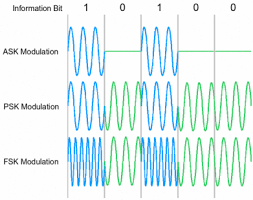
\includegraphics[scale=0.8]{vormen van modulatie.png}
\caption{Vormen van modulatie}
\end{figure}

\subsubsection{Phase Shift Keying 'PSK,QPSK'}

Er zijn verschillende methodes van PSK zoals:
\begin{itemize}
  \item Binaire Phase Shift Keying (`BPSK') $\Rightarrow$ 1-bit symbool
  \item Quadrature Phase Shift Keying (`QPSK') $\Rightarrow$ 2-bit symbool
  \item Enzv.
\end{itemize}

BPSK is de eenvoudigste vorm van PSK met '1 bit per symbool'. Het constellatiediagram (IQ) van BPSK ziet er als volgt uit:
\begin{itemize}
  \item Een '1' $\Rightarrow$ 0°
  \item Een '0' $\Rightarrow$ 180°
\end{itemize}

\begin{figure}[H]
\centering
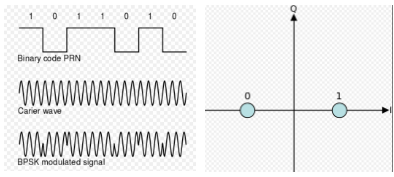
\includegraphics[scale=0.8]{BPSK.png}
\caption{BPSK}
\end{figure}

\begin{figure}[H]
\centering
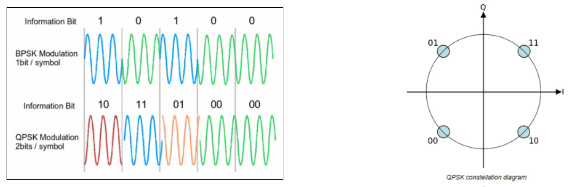
\includegraphics[scale=0.8]{QPSK.png}
\caption{Quadrature Phase Shift Keying}
\end{figure}

\subsubsection{Klokextractie}

Klokextractie vs. Demodulatie
\begin{itemize}
  \item Om de verzonden data uit het gemoduleerde signaal te kunnen halen, is het noodzakelijk om de klokfrequentie waarmee verzonden is te kennen, de 'sample frequentie'.
  \item Dit proces noemen we klokextractie, waarbij de ontvanger wordt gesynchroniseerd met de zender.
  \item Wanneer er voldoende veranderingen in het gemoduleerde signaal aanwezig zijn, is het mogelijk de zendklok te extraheren uit het gemoduleerde signaal. De veranderingen in het gemoduleerde signaal corresponderen namelijk met de zendklok frequentie.
\end{itemize}

Klokextractie vs. Preamble
\begin{itemize}
  \item In de preamble kan vaak ook de klokfrequentie worden verkregen.
  \item Wat is dan een Preamble?
\end{itemize}

Voor een goede demodulatie is het dus noodzakelijk dat de ontvangstklok dezelfde frequentie krijgt als de zendklok. Nog belangrijker is dat de fase van de ontvangstklok in orde is!


\subsubsection{Quedrature Amplitude Modulation 'QAM'}
PSK is praktisch te gebruiken met maximaal 8 fases. Om meerdere levels te kunnen gebruiken wordt QAM toegepast.
Hierbij wordt een combinatie van amplitude en fasesprongen
gemaakt.

\begin{figure}[H]
\centering
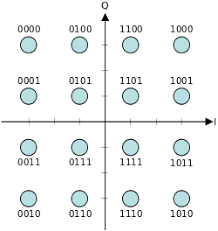
\includegraphics[scale=0.8]{Constelatiediagram.png}
\caption{Constellatie}
\end{figure}

\begin{figure}[H]
\centering
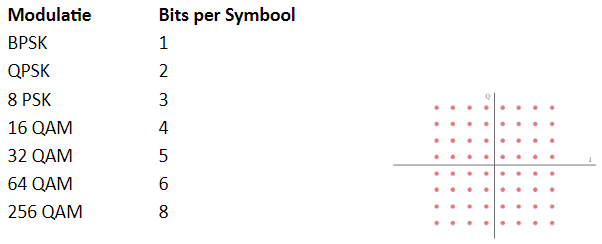
\includegraphics[scale=0.8]{Digitale modulatie overzicht.png}
\caption{Digitale modulatie: overzicht}
\end{figure}


\subsubsection{Transmissiepad en Parameters}

\begin{itemize}
    \item Zendvermogen: Het uitgangsvermogen van de zendunit, meestal
    uitgedrukt in dBm.
    \item RSSI ‘Received Signal Strength Indicator’: Het gemeten
    ontvangstniveau in de ontvangstunit. Meestal uitgedrukt in dBm.
    Met meer symbolen krijg je ook een hogere RSSI
    \item Receive Level: Meestal wordt hier een range mee aangeduid
    waarbinnen het ontvangstniveau moet liggen.
    \item S/R: ratio geeft de Signal to Noise Ratio aan. Meestal wordt van de
    ontvanger opgegeven welke S/R nodig is om een bepaalde BER te
    garanderen. De S/R wordt uitgedrukt in dB.
    \item Bandwidth: De bandbreedte van het RF signaal dat uit de zender
    komt.
    \item  BER: Bit Error Rate is de verhouding tussen het aantal foute
    ontvangen bits ten opzichte van het totaal aantal ontvangen bits.
    BER = (aantal foutieve bits) / (totaal aantal ontvangen bits)
    \item Interference: Verstoring van het ontvangstsignaal door andere
    zenders of door multipathfading.
    \item Attenuation (verzwakking): Demping die optreedt door bijvoorbeeld
    kabels, connectoren en de free space los.
    \item Phasedistortion: Fasevervorming die ontstaat door een verschil in
    looptijd(snelheid) van de aanwezige frequentiecomponenten in een
    pulsvorming signaal (dispersie).
  \end{itemize}


\subsubsection{LoRa}

\begin{figure}[H]
\centering
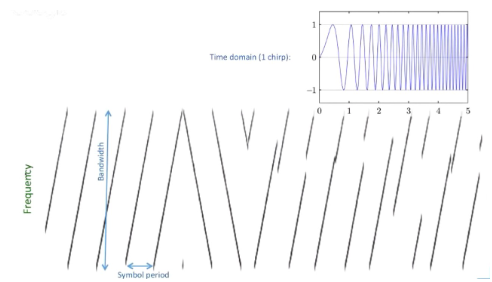
\includegraphics[scale=0.8]{LoRa chirp.png}
\caption{LoRa}
\end{figure}

\begin{figure}[H]
\centering
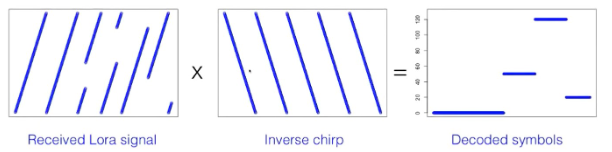
\includegraphics[scale=0.8]{LoRa Demodulatie.png}
\caption{LoRa}
\end{figure}


    \subsection{les 4 Antennetheorie}
    Date : 19 januari 2024\\

De radiogolf (elektromagnetische golf) ondervindt de volgende verstoringen:
\begin{itemize}
  \item Absorptie: Vooral bij frequenties boven 4 GHz.
  \item Diffractie: Verstoring door objecten in het radiopad.
  \item Obstructie: Onderbreking van het signaal door een object.
  \item Multipath fading: Ongewenste reflecties van het radiosignaal die bij de ontvanger binnenkomen via een andere weg.
  \item Reflecties via ionosfeer en troposfeer (f < 30 MHz).
  \item Free Space Path Loss, vrije ruimte demping.
\end{itemize}

\begin{figure}[H]
    \centering
    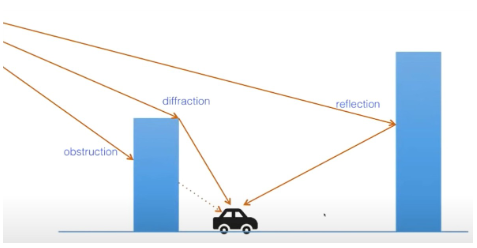
\includegraphics[scale=0.8]{Multipath fading1.png}
    \caption{multipathfading}
    \end{figure}

\begin{figure}[H]
    \centering
    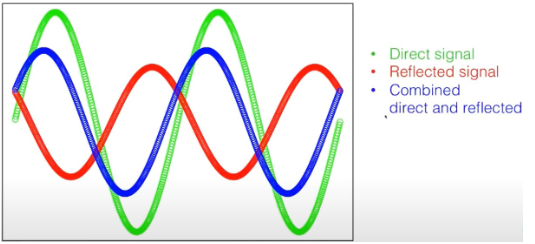
\includegraphics[scale=0.8]{Multipath fading2.png}
    \caption{multipathfading}
    \end{figure}

\begin{figure}[H]
    \centering
    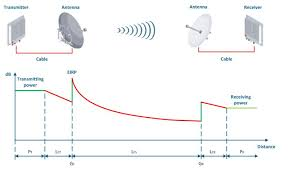
\includegraphics[scale=0.9]{link budget.jpeg}
    \caption{Link Budget}
    \end{figure}

\subsubsection{Free Space Path Loss}

\begin{figure}[H]
    \centering
    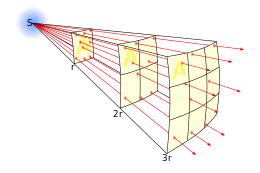
\includegraphics[scale=0.8]{free path space loss.png}
    \caption{free path space loss}
    \end{figure}

Het bereik van een draadloze verbinding wordt in grote mate beperkt door de Free Space Path Loss (FSPL).
\begin{itemize}
    \item Er gaat geen energie verloren, maar de energie verdeelt zich over het oppervlak.
    \item Bij FSPL wordt uitgegaan van een isotrope straler.
    \item Deze antenne straalt het signaal in alle richtingen met gelijke sterkte uit.
\end{itemize}

\begin{figure}[H]
    \centering
    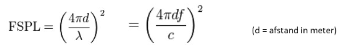
\includegraphics[scale=0.8]{FSPL.png}
    \caption{FSPL Formule.}
    \end{figure}

Wat is de FSPL(dB) voor een frequentie van 434 MHz en van 868 MHz op bijv. een afstand van 500 meter?\\
Wat valt je op aan het antwoord?\\
434 MHz = 79,2 dB\\
868 MHz = 85,2 dB\\
Een frequentieverdubbeling leidt tot 6dB (vierdeling) extra demping.

\subsubsection{Antenne}
De antenne zorgt voor: De uitstaling van de radiogolf in de gewenste richting, daardoor mogelijk ook voor compensatie van de FSPL. (De energie wordt gebundeld)\\

Een antenne heeft de volgende kenmerken:
\begin{itemize}
  \item Ingangsimpedantie
  \item Gain en stralingsdiagram (radiation pattern)
  \item Afmeting
  \item Resonantiefrequentie
\end{itemize}

Antenne impedantie

De antenne is te beschouwen als een resonantiekring.
\begin{itemize}
  \item Op de resonantiefrequentie is de impedantie in Ohms. Deze impedantie wordt bepaald door het type antenne en het gebruikte materiaal. Veelvoorkomend is een impedantie van 50 Ohm.
  \item Belangrijk is dat deze impedantie overeenkomt met de feeder (kabel) impedantie en de zender/ontvanger impedantie. Wanneer deze impedantie niet overeenkomt, treedt er reflectie op.
\end{itemize}

\begin{figure}[H]
    \centering
    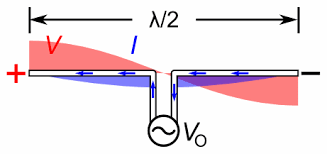
\includegraphics[scale=0.8]{halve golf resonantie.png}
    \caption{De halve golf dipoolantenne in resonantie}
    \end{figure}

We beperken ons tot een veelgebruikt type: de halve golf dipool. De lengte is ongeveer \(0,95 \times \frac{\lambda}{2}\) (de \(0,95\) is de verkortingsfactor van het antennemateriaal).
In een medium is \(\lambda = \frac{c \cdot k}{f}\) (waarbij \(k\) de verkortingsfactor van het materiaal van de antenne is).\\

De polarisatie wordt bepaald door de positie van de straler (dipool),
deze bepaald het elektrische veld.
Typen polarisatie: Horizontaal, verticaal, circulair

\newpage

\section{Laagfrequent}

    \subsection{les 1 Voedingsconcepten}
    date : 5 december 2023

\subsubsection*{Ontwerp Parameters van Voedingen}

\begin{enumerate}[label=--]
  \item \textbf{Ingangsspanning:} \\
    Beschrijving van de vereiste ingangsspanning voor de voeding.

  \item \textbf{Uitgangsspanning:} \\
    Beschrijving van de gewenste uitgangsspanning van de voeding.

  \item \textbf{Dissipatie en Rendement:} \\
    Specificatie van de dissipatie en het rendement van de voeding.

  \item \textbf{Ruis:} \\
    Beschrijving van de gewenste niveaus van ruis in de voeding.

  \item \textbf{Inschakelverschijnselen:} \\
    Verklaring van de verschijnselen die optreden bij het inschakelen van de voeding.

  \item \textbf{Uitschakelverschijnselen:} \\
    Verklaring van de verschijnselen die optreden bij het uitschakelen van de voeding.
\end{enumerate}

\begin{figure}[H]
\centering
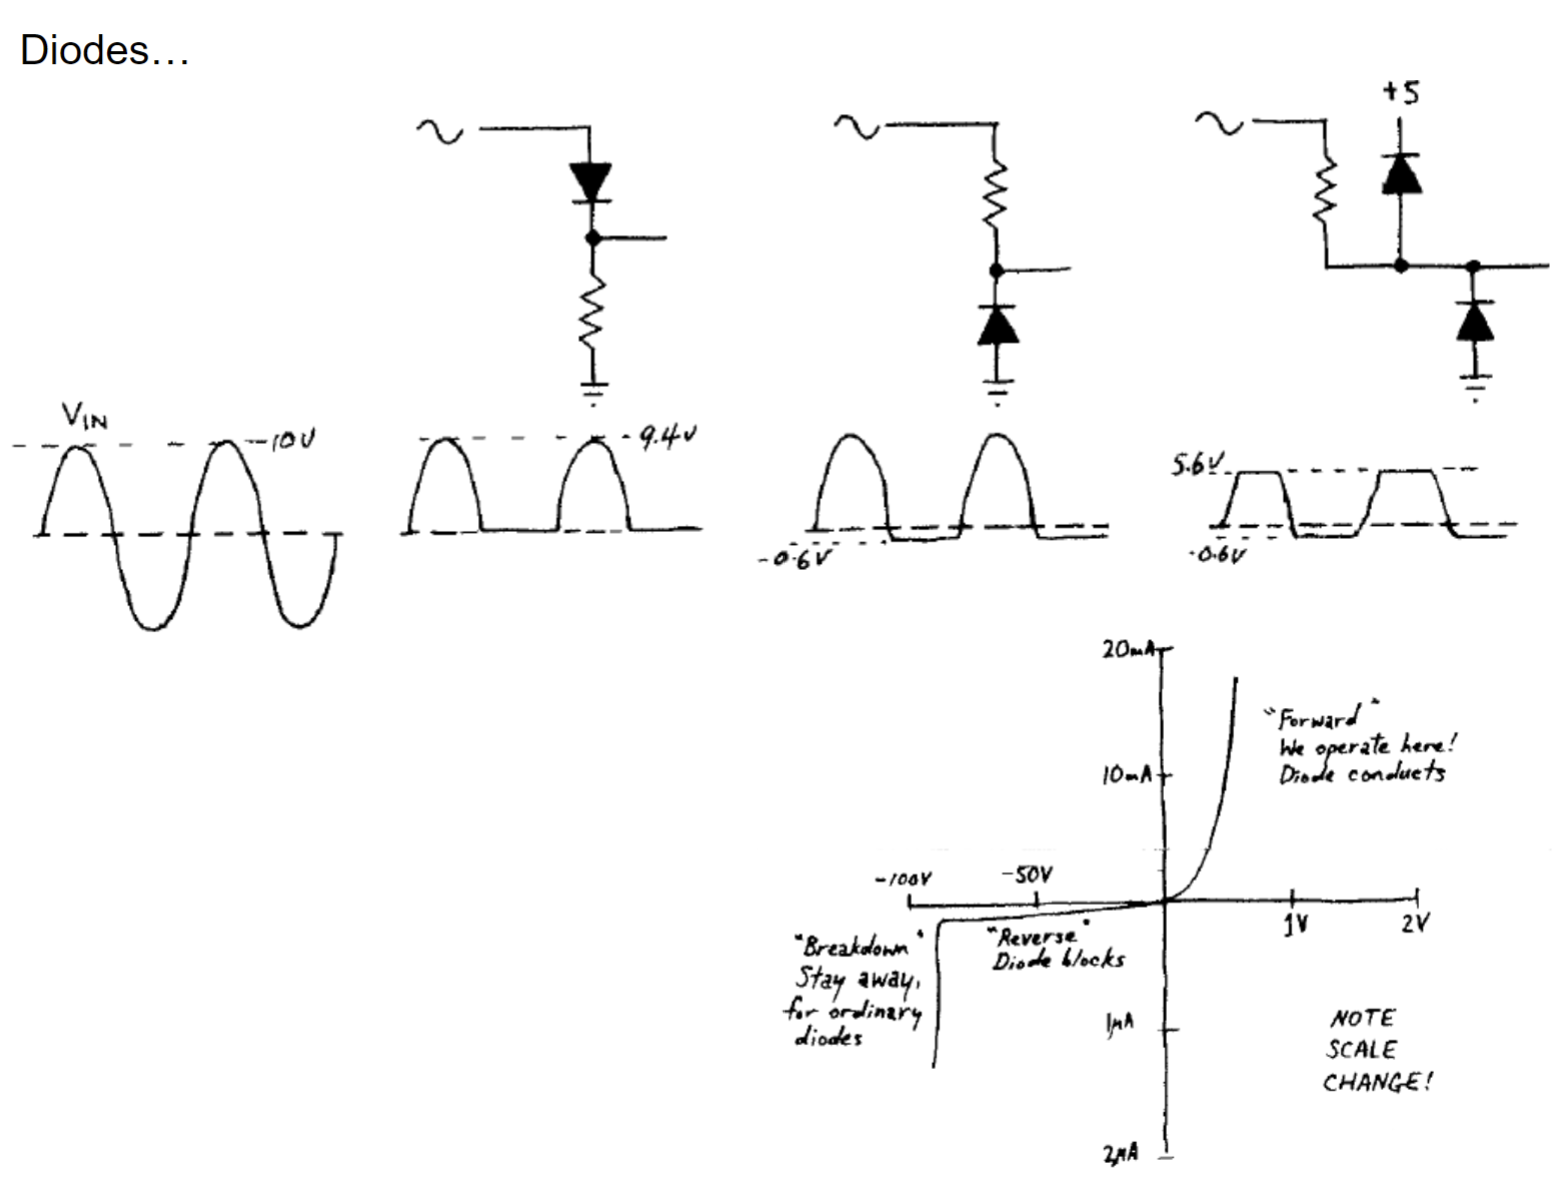
\includegraphics[scale=0.5]{Diode.png}
\end{figure}

\subsubsection*{Verschil tussen een Normale Diode en een Zener-diode}

Een \textbf{normale diode} en een \textbf{Zener-diode} zijn beide halfgeleiderapparaten die stroom in één richting laten stromen. Het belangrijkste verschil tussen deze twee typen diodes ligt in hun gedrag bij omgekeerde polarisatie.\\

Een normale diode laat stroom in slechts één richting toe en blokkeert stroom in de omgekeerde richting. Wanneer de diode in de omgekeerde richting wordt gepolariseerd boven een bepaalde spanning, zal er een punt komen waarop de diode zal doorslaan en stroom gaat geleiden in omgekeerde richting. Dit wordt het \textit{omgekeerde knelpunt} genoemd en moet worden vermeden in normale toepassingen.\\

Een Zener-diode is ontworpen om bewust te werken in de omgekeerde doorslagregio. De belangrijkste eigenschap van een Zener-diode is het handhaven van een vrijwel constante spanning over zijn terminals, zelfs wanneer deze in omgekeerde polarisatie is aangesloten en het omgekeerde knelpunt heeft bereikt. Deze constante omgekeerde spanning wordt de \textit{Zener-spanning} genoemd.\\

In toepassingen wordt een Zener-diode vaak gebruikt als spanningsregelaar, waarbij het stabiele Zener-spanningsniveau wordt gebruikt om een constante uitgangsspanning te handhaven.

\subsubsection*{DC/DC Converters}
\begin{figure}[H]
    \centering
    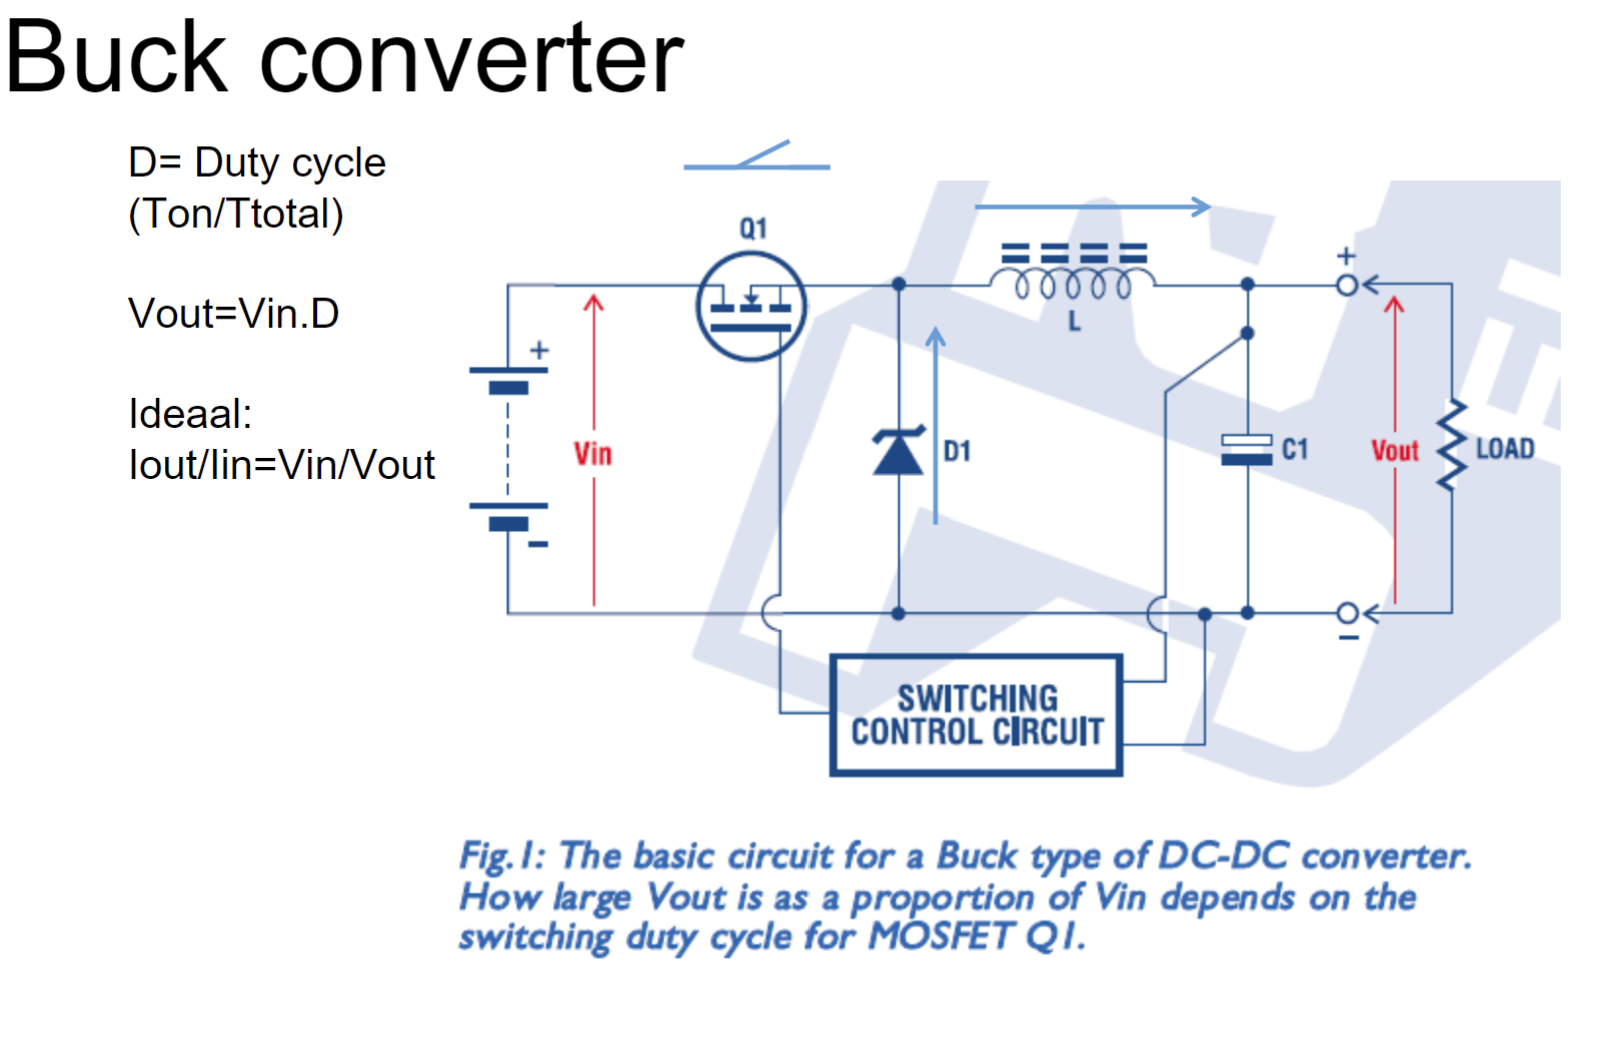
\includegraphics[scale=0.5]{Buck.png}
    \caption*{ non isolated spannings verlager}
    \end{figure}
\begin{figure}[H]
    \centering
    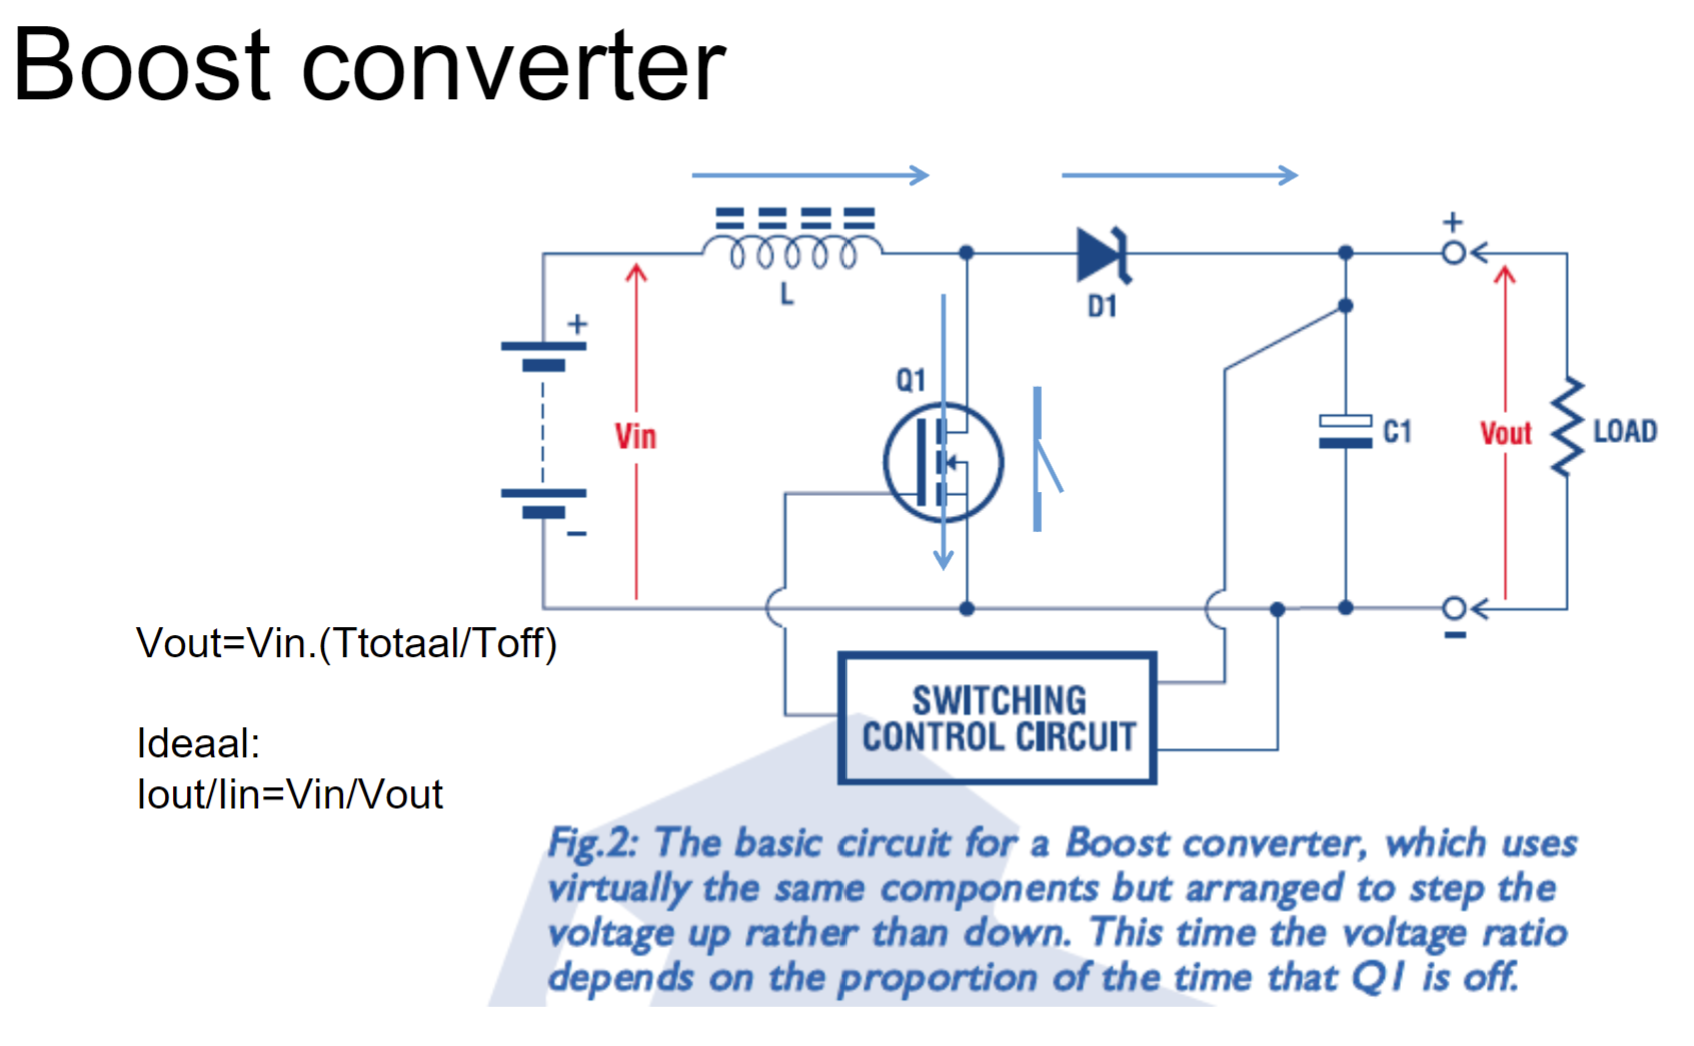
\includegraphics[scale=0.5]{boost.png}
    \caption*{ non isolated spannings verhoger}
    \end{figure}
\begin{figure}[H]
    \centering
    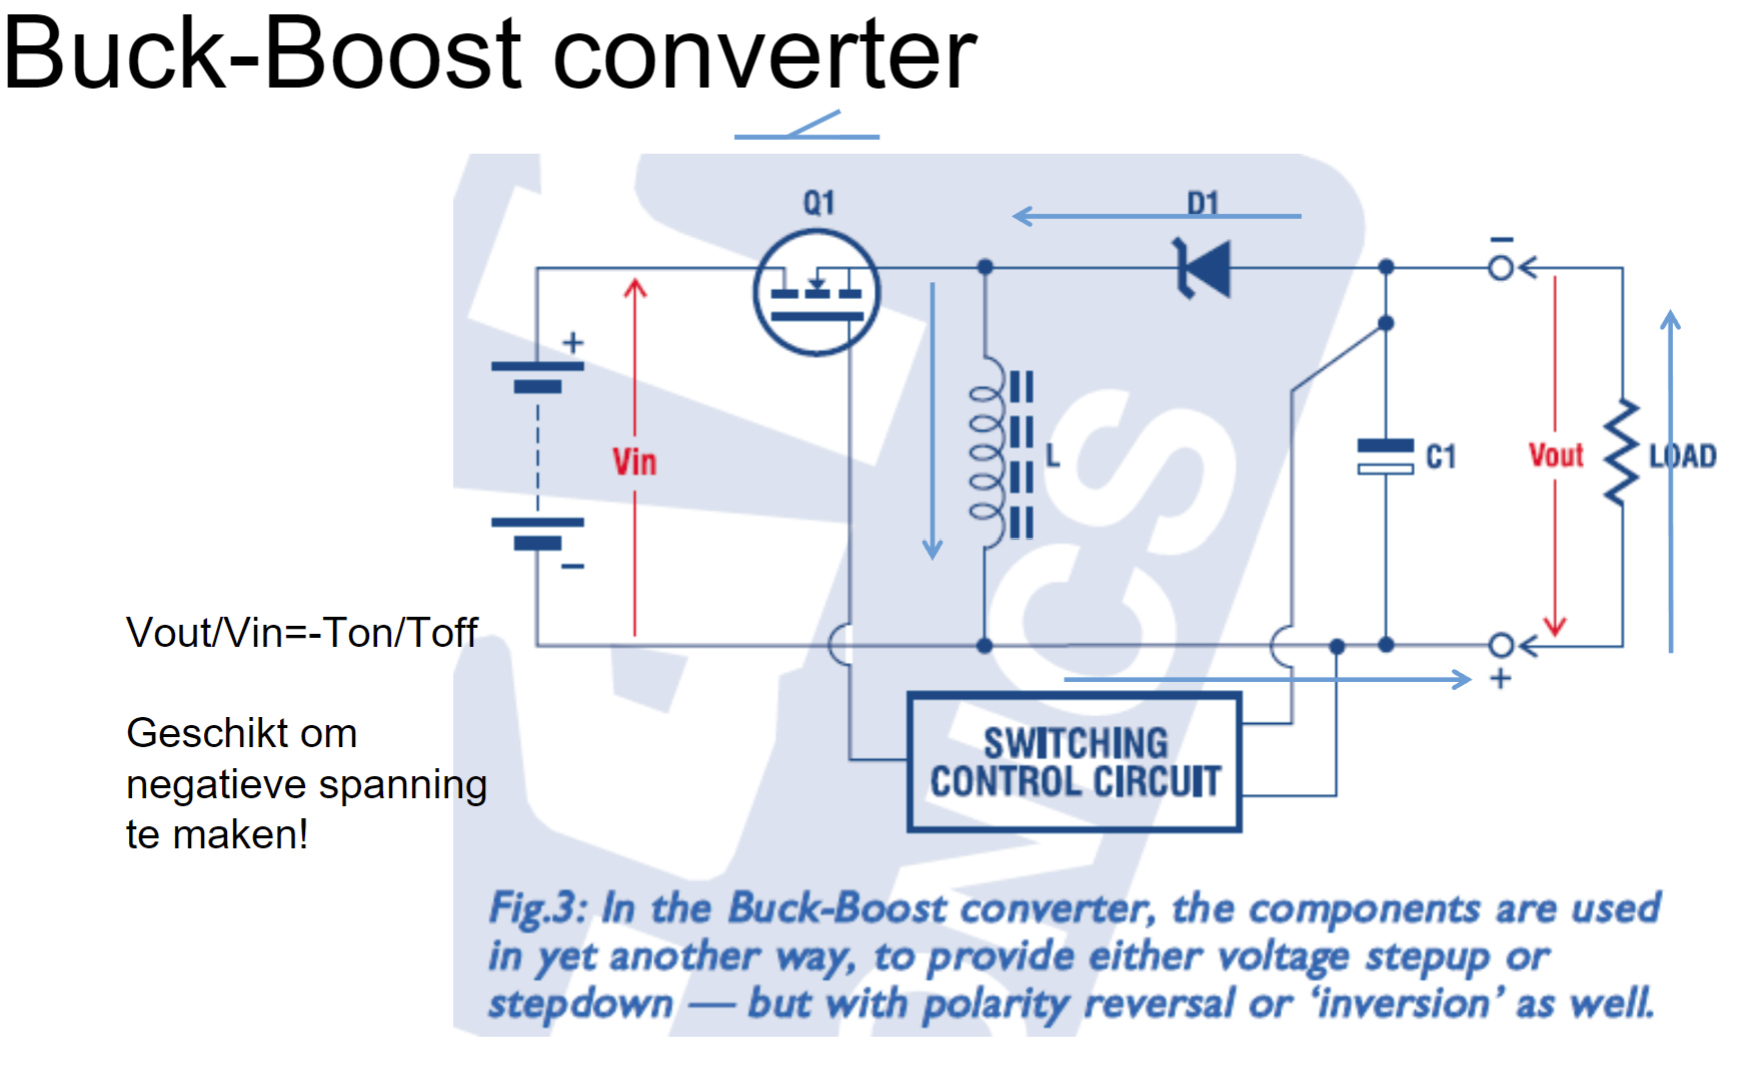
\includegraphics[scale=0.5]{buck-boost.png}
    \caption*{ non isolated spannings verhoger en verlager}
    \end{figure}
\begin{figure}[H]
    \centering
    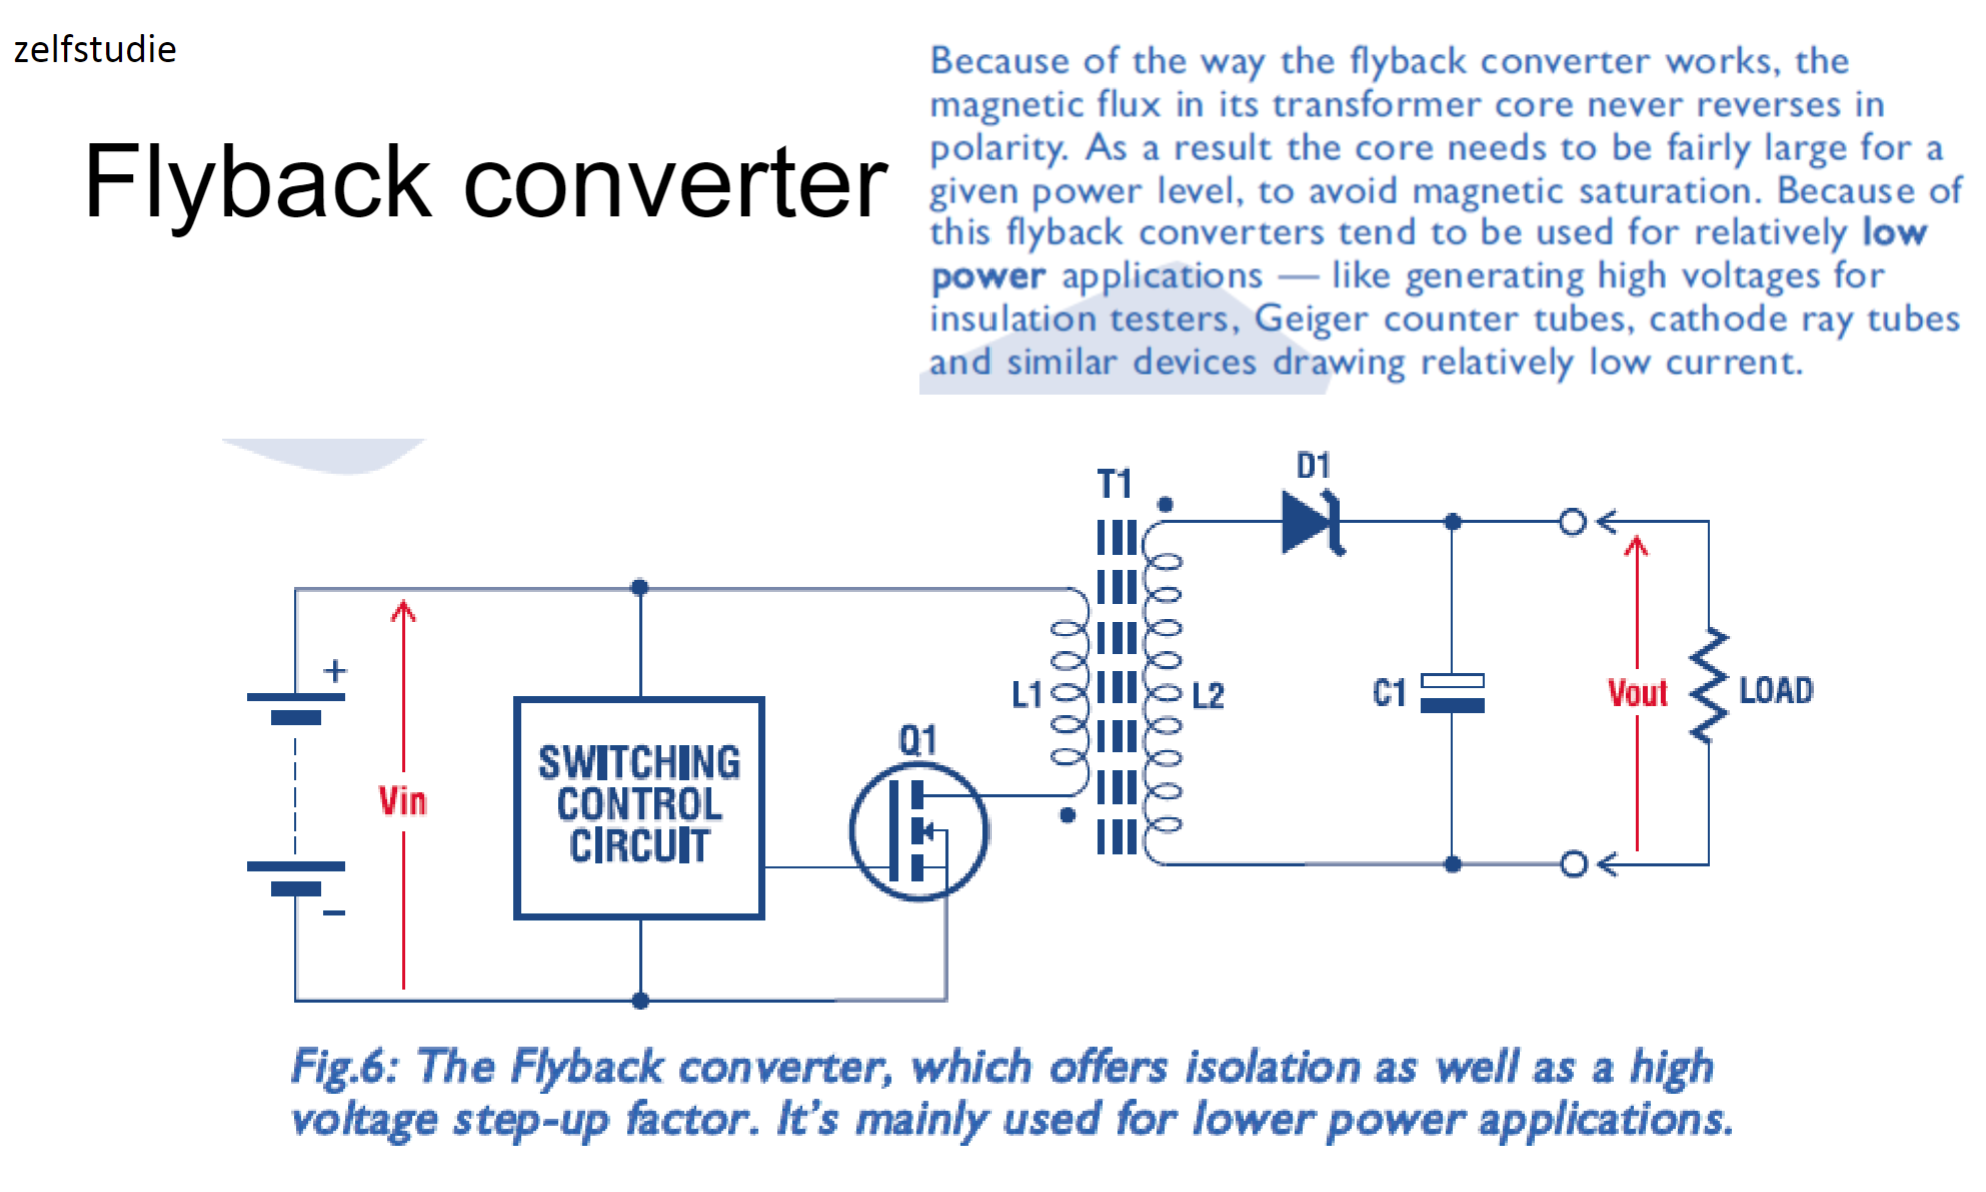
\includegraphics[scale=0.5]{flyback.png}
    \caption*{ Isolated converter Flyback}
    \end{figure}
\begin{figure}[H]
    \centering
    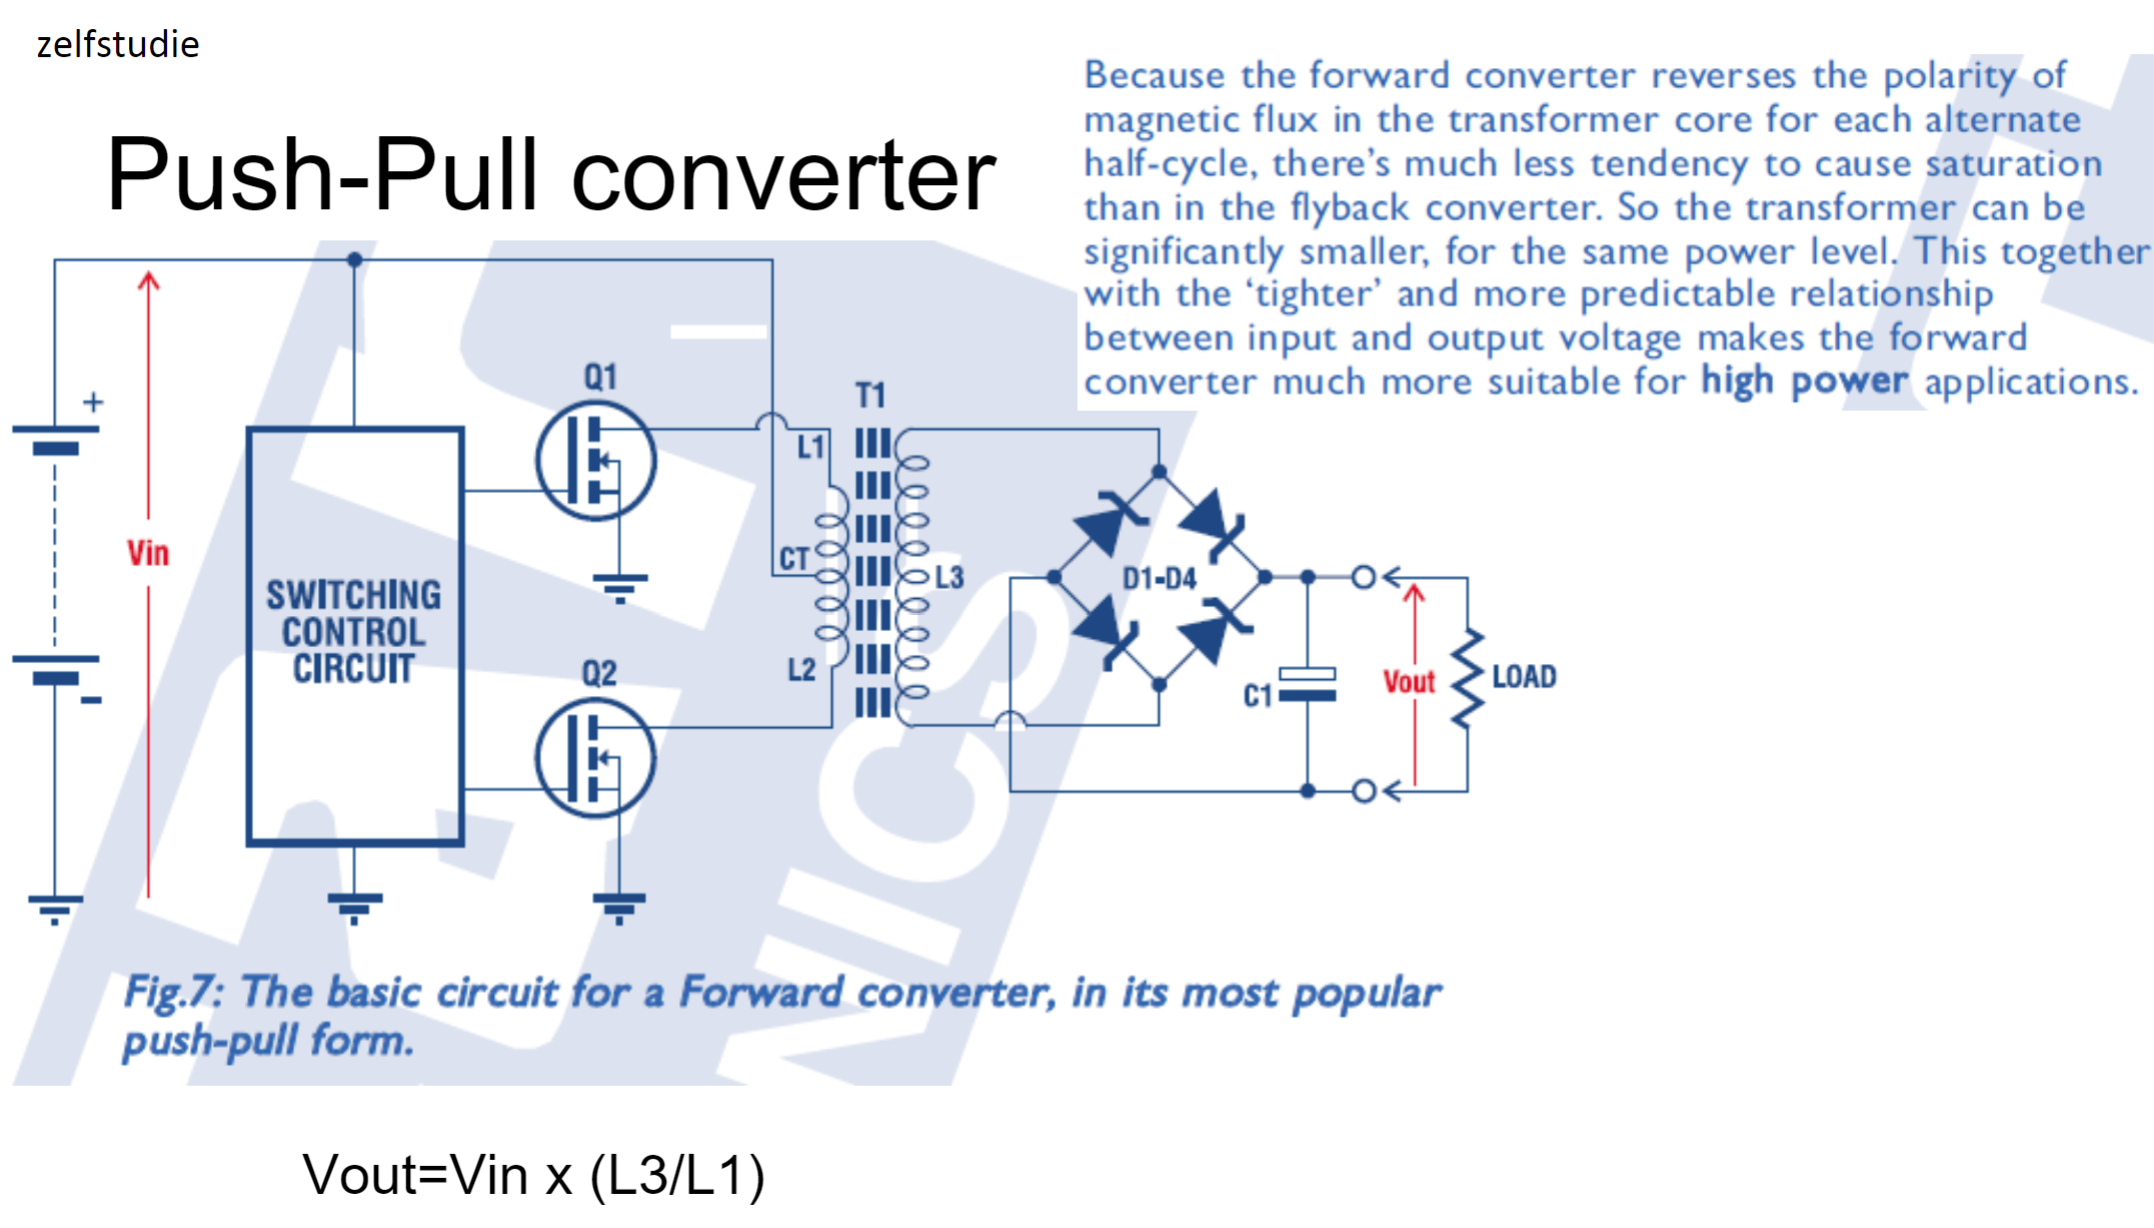
\includegraphics[scale=0.5]{push-pull.png}
    \caption*{ Isolated converter push pull}
    \end{figure}


Verbeteringen
\begin{itemize}
    \item Synchronous rectification
    \item Overal waar een diode staat -> geschakelde mosfet
    \item Clock sync
\end{itemize}
Hogere frequenties
\begin{itemize}
    \item Nieuwe materialen!
    \item Maakt kleinere converters mogelijk....
\end{itemize}

\vspace{1cm}
Switcher of LDO??\\
Switcher:
\begin{itemize}
    \item Betere efficiëntie
    \item Blijft koel
    \item Kan van zo ongeveer alle Uin alle Uout maken
    \item Zeer nauwkeurig PCB plan
\end{itemize}
LDO:
\begin{itemize}
    \item Geen storende frequenties door schakelen
    \item Single chip Solutions (op de Cap na!)
    \item Goedkoop
    \item Rendement is relatief laag (Udrop out bepaald minimum)
\end{itemize}


    \subsection{les 2 Low power design}
    date : 12 december 2023

Waar zit de start van een low power ontwerp?
\begin{itemize}
    \item In kaart brengen van de duur en piek van het vermogens verbruik
    \item fysieke grootte
    \item I/O vraag
    \item Aan/uit tijd
    \item opladen?
\end{itemize}

\vspace{0.5cm}
Wat te doen om batterij te sparen?
\begin{itemize}
    \item Geen optische interfaces.
    \item gebruik geen relais. Alleen solid state relais als het echt nodig is.
    \item geen backlight als het geen eis is.
    \item zo min mogelijk leds
    \item zo min mogelijk IO.
    \item Snelheid is een killer. Dubbele Snelheid is dubbel vermogen.
\end{itemize}

\vspace{0.5cm}
Wat kan uit\dots
\begin{itemize}
    \item Denk na over duty cycle of use.
    \item stablisatie na inschakelen?
    \item meer vermogen voor beheersing van power.
    \item zijn pull-up weerstanden altijd nodig? mag het ook met pull down?
    \item power buffers - line buffers.
    \item let op diode kruip-paadjes
    \item kunnen de
    \begin{itemize}
        \item opamps
        \item DA converters
        \item Stroombronnen
        \item Processoren
    \end{itemize}
    uit en hoe gaan ze weer aan?
\end{itemize}

\vspace{0.5cm}
Selectie vragen voeding.
\begin{itemize}
    \item Wat voor spanning is nodig?
    \item Moet de batterij oplaadbaar zijn?
    \item Hoe ziet de gebruiks/laad cycle eruit voor dit roduct?
    \item Wat is het piekverbruik van het system?
    \item Moet de batterij eenvoudig vervangbaar zijn?
    \item laden en simultaan gebruiken van de accu?
\end{itemize}

\begin{figure}[H]
    \centering
    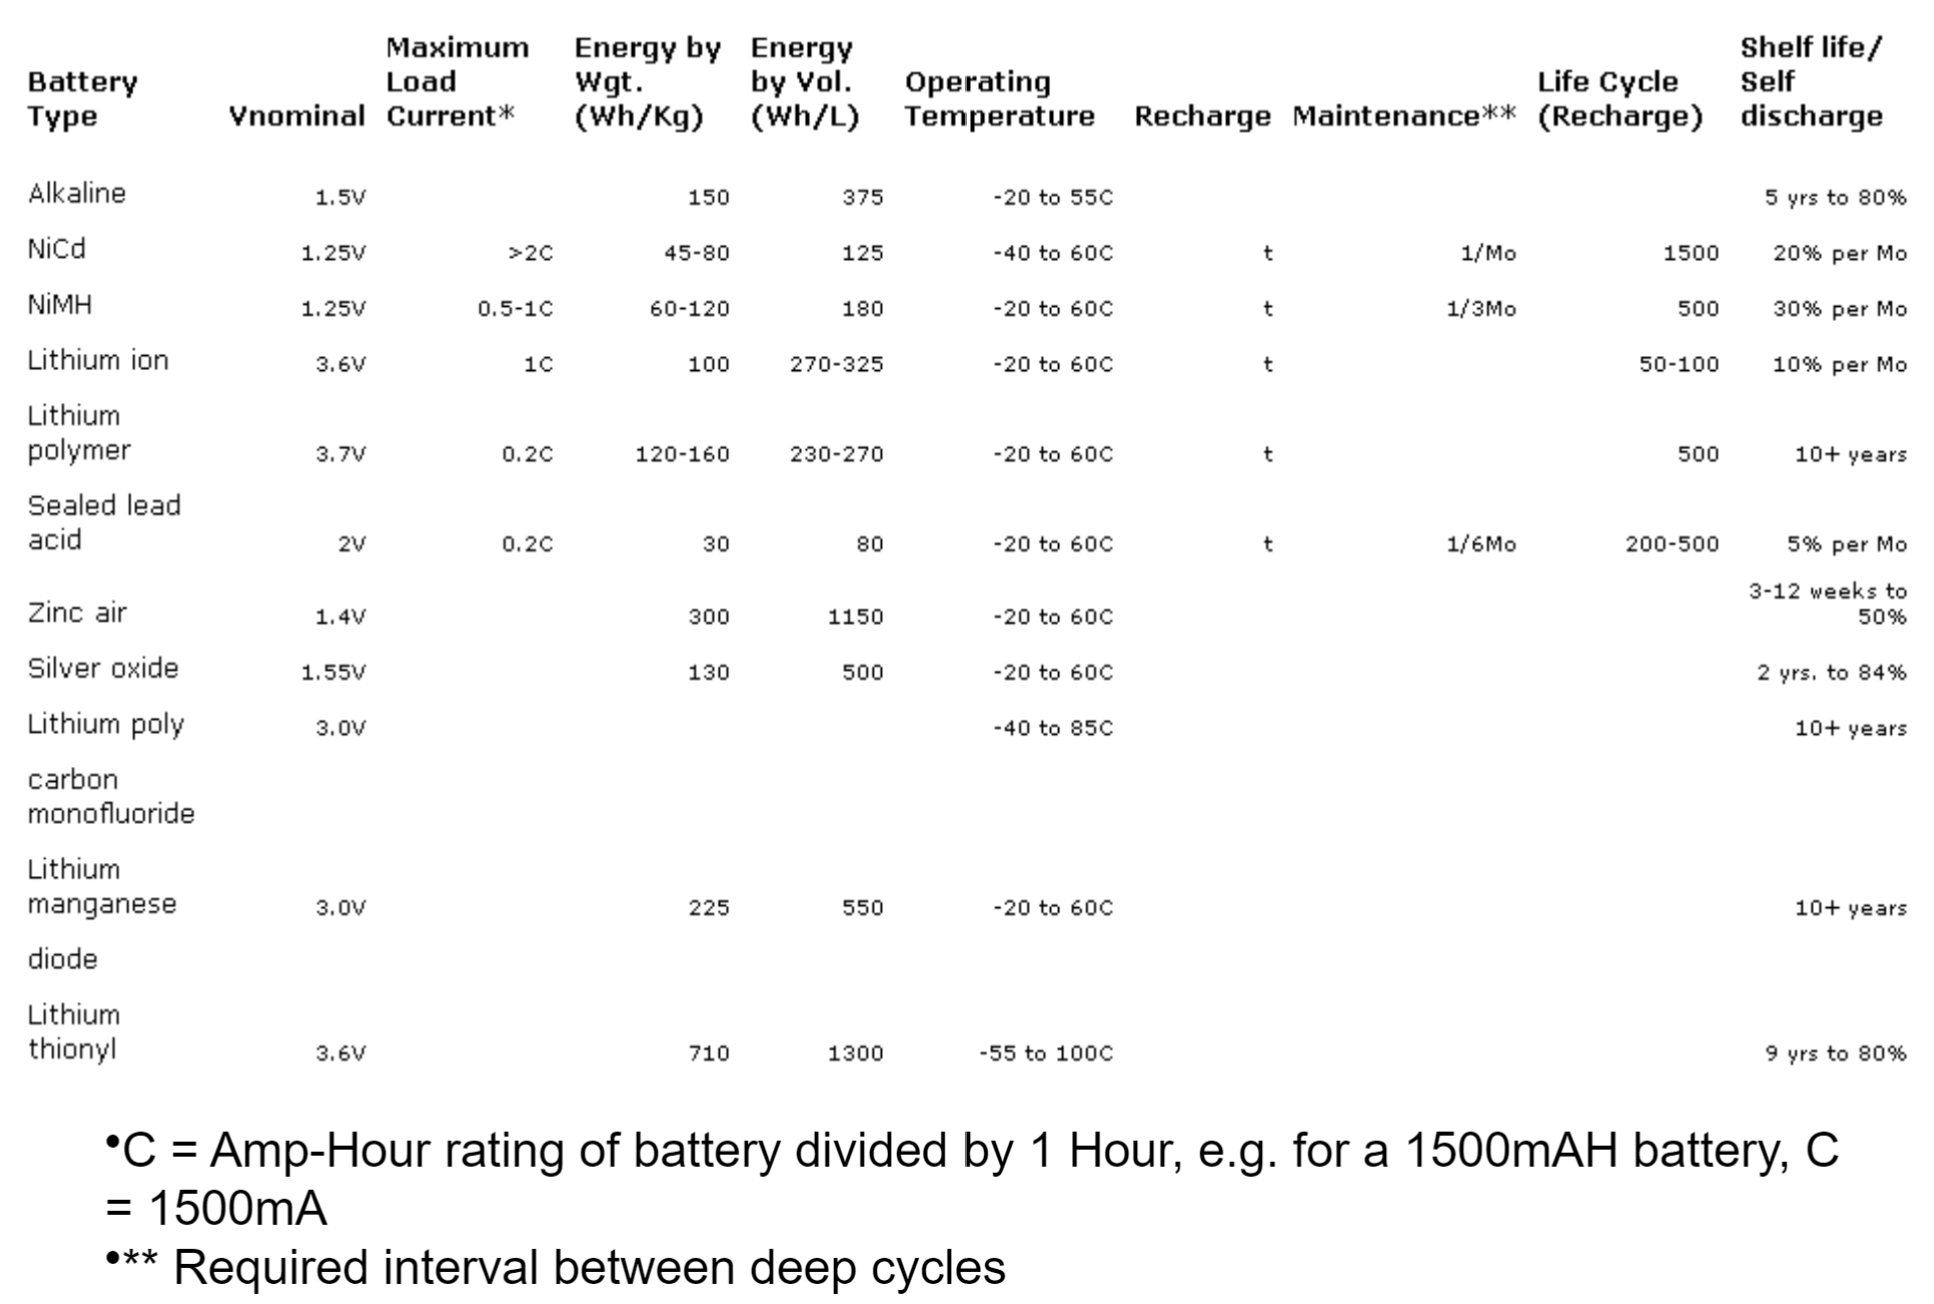
\includegraphics[scale=0.5]{batterijen.png}
    \caption*{ soorten batterijen}
    \end{figure}


    \subsection{les 3 Interfaces}
    date : 9 januari 2024

Data communicatie:\\
simplex: van A naar B\\
Half -duplex: van A naar B of B naar A\\
Full-duplex: Van A naar B en B naar A.

Een synchroom signaal stuur ook een referentie klok mee.

\subsubsection{I2C}
\begin{itemize}
    \item two wired bus: SDA (data) en SCL (clock) <- (dus synchroom)
    \item originally to interact within small numbers of chips
    \item speeds:
    \begin{itemize}
        \item 100 kbps (standard mode)
        \item 400 kbps (fast mode)
        \item 3.4 Mbps (high-speed mode)
    \end{itemize}
    \item data transfer: serial, 8-bit oriented, bi-directional (Half-duplex)
    \item master/slave relationship wiht multi-master option
    \item master can operate as transmitter or receiver
    \item addressing: 7 bit or 10 bit unique addresses
    \item device count limit : max. capacitance 400pF
\end{itemize}

\begin{figure}[H]
    \centering
    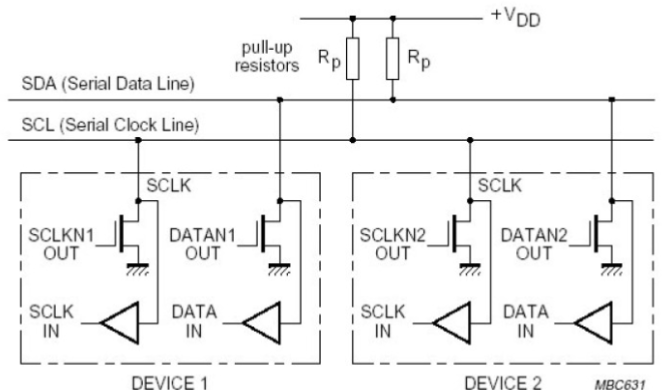
\includegraphics[scale=0.7]{i2c.png}
    \caption*{ I2C}
    \end{figure}

\begin{figure}[H]
    \centering
    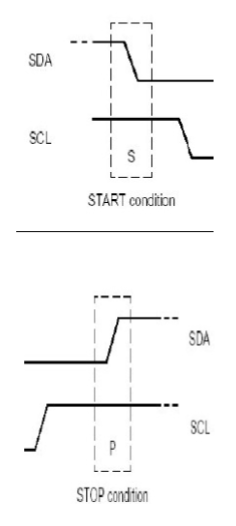
\includegraphics[scale=0.7]{i2c start stop.png}
    \caption*{start stop signaal van I2C}
    \end{figure}

\begin{figure}[H]
    \centering
    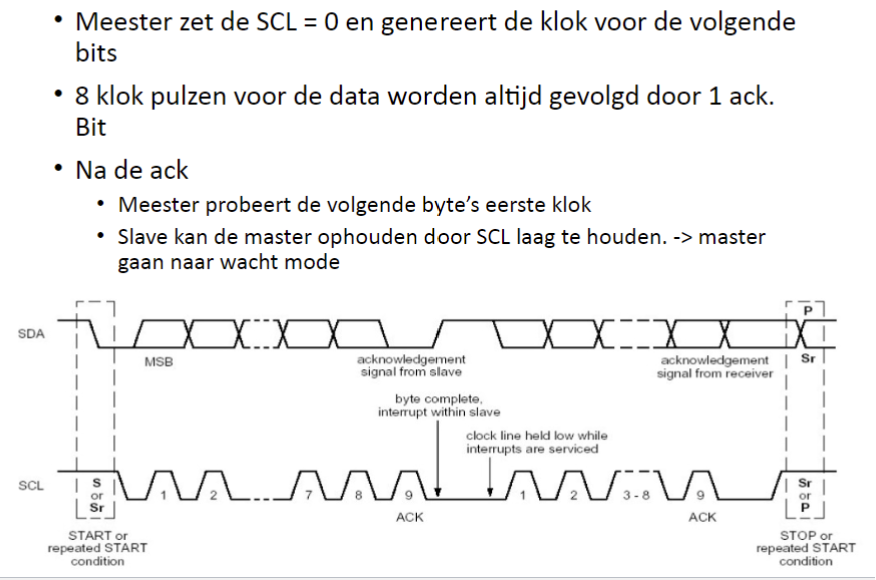
\includegraphics[scale=0.7]{Data transfer i2c bus.png}
    \caption*{Data transfer I2C bus}
    \end{figure}

Bij de 9de scl puls moet de slave de sda laag houden om te acken. Slave moet SDA ook weer loslaten na de ack
(neergaande klok).

\begin{figure}[H]
    \centering
    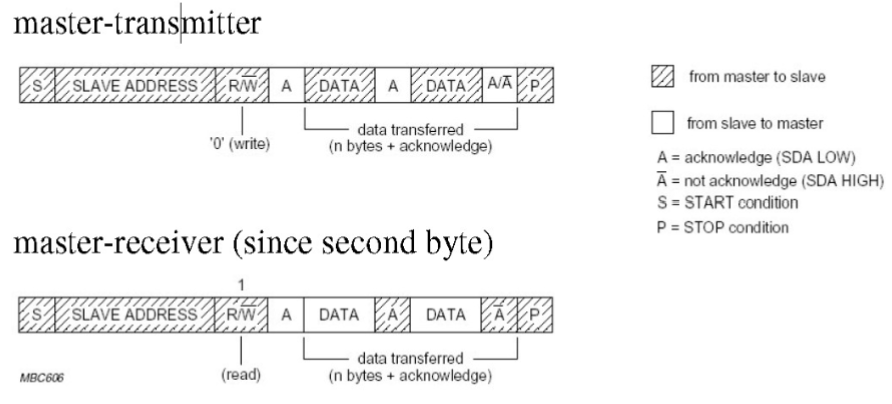
\includegraphics[scale=0.7]{Frame Format.png}
    \caption*{Frame format van I2C}
    \end{figure}

\subsubsection{1-Wire}
\begin{figure}[H]
    \centering
    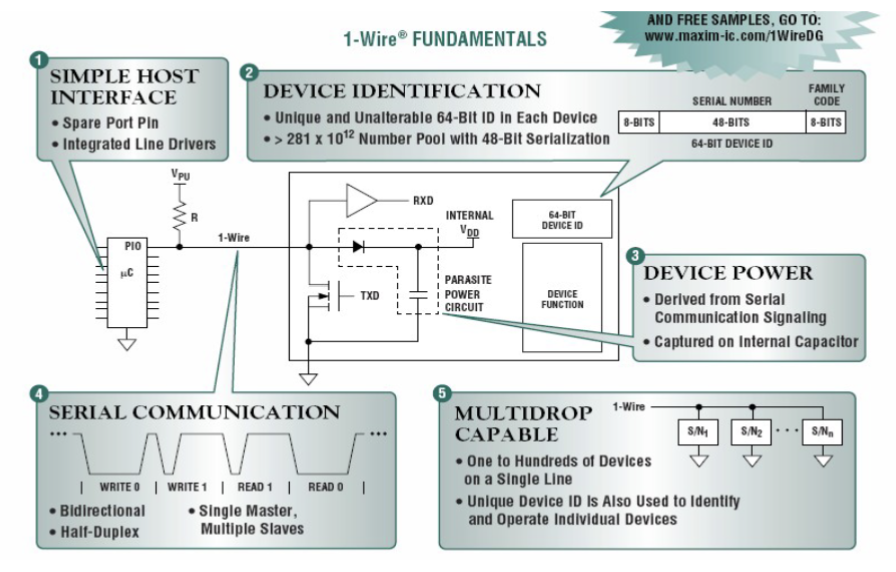
\includegraphics[scale=0.7]{1wire fundemental.png}
    \caption*{1-Wire Fundementals}
    \end{figure}

Wat is 1-wire?
\begin{itemize}
    \item Low-cost micro Lan.
    \item Digital communicatie over twisted pair
    \item globale opbouw.
    \begin{itemize}
        \item Open drain master/slave multidrop
        \item max 1 master
        \item Slave, dus 'spreek meester' en dan pas antwoorden.
        \item communicatie tussen slaves alleen mogelijk via de master.
    \end{itemize}
    \item trager dan I2C maar wel grotere afstanden <100m
    \item Standaard mode 15kbps in onverdrive 111kbps
\end{itemize}

\vspace{0.5cm}
Eigenschappen protocol
\begin{itemize}
    \item 64 bit uniek addresses8x8 bits
    \item start met LSB
    \item Eersste 8 bits familie code en identificatie
    \item Volgende 6*8 bits vormen een uniek nummer
    \item Laatste  bits is een CRC van de 1e byte ter verificatie
    \item aantal adressen dus 2 tot de macht 48 zijn er heel veel.
\end{itemize}

\begin{figure}[H]
    \centering
    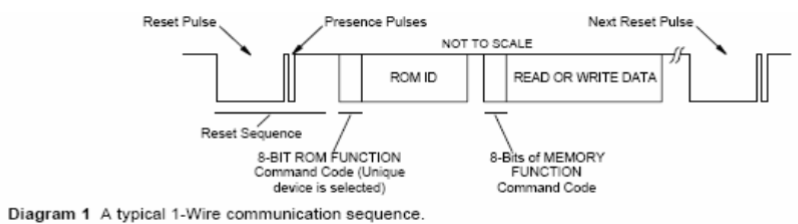
\includegraphics[scale=0.7]{1wire communicatie.png}
    \caption*{1-Wire communication}
    \end{figure}

\subsubsection{SPI van Motorola}
\begin{itemize}
    \item Geen protocol op de lijn
    \item In vergelijk met I2C snel
    \item synchroomMaster nodes in chipsFull duplex mogelijk
    \item adresseren met de slave select
\end{itemize}

Inerface bestaat uit:\\
SCLK: de klok.\\
MOSI: van de master naar de slave.\\
MISO: van de slave naar de master.\\
SSC of SS: Slave select.

\subsubsection{AMBA Bus}
\begin{figure}[H]
    \centering
    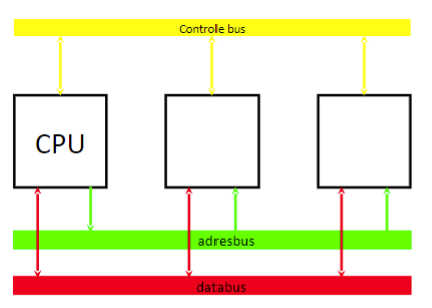
\includegraphics[scale=0.7]{AMBA bus.png}
    \caption*{AMBA Bus}
    \end{figure}

AMBA Bus wordt gebruikt voor SoC's. SoC's zijn system on chip designs overterwijl chip+software+integration.

\vspace{0.5cm}
AMBA (Advanced Microcontroller Bus Architecture) is a collection of buses from ARM for stisfying a range of different criteria.

APB (Advanced Peripheral Bus): simple strobed-acces bus with minimal interface complexity. Suitable for hosting peripherals.
\begin{itemize}
    \item Is geoptimaliseerd voor minimale vermogensopname
    \item Vereendvoudige opbouw van het businterface
    \item Relatieve lage bandbreedte t.o.v. de AHB of ASB
    \item Geen piplined operations
    \item Nieuwste versie APB relateert alle operaties t.o.v. de opgaande flank
    \item lage belasting AHB of ASB door toepassing van een APB bridge
\end{itemize}

ASB (Advanced System Bus): a multimaster synchronous system bus.

AHB (Advanced High Performance Bus): a high- throughput
synchronous system backbone. Burst transfers and split transactions.
\begin{itemize}
    \item 4 logische elementen:
    \begin{itemize}
        \item master
        \item slave
        \item arbitter
        \item decoder
    \end{itemize}
    \item meerdere busmasters
    \item split transactions :Een slaafje met een lange response tijd kan tijdens het decoderen van de opdracht de bus
    loslaten en een ander proces laten passeren. Hierna is het tijd voor het eerste slaafje als hij zijn
    werkje klaar heeft
    \item single clock edge operation: Heel handig wanneer je timing analyse aan de gang gaat. Hiermee is het mogelijk om je ontwerp
    te controleren en te verifiëren
    \item non-tristate implementation: Gebruik van een centrale gemultiplexte bus.
    \item variable bus bredte 16,32,64,128 bits
\end{itemize}

• One solution to the design productivity gap is to make ASIC designs
more standardized by reusing segments of previously manufactured
chips.

• These segments are known as “blocks”, “macros”, “cores” or “cells”.

• The blocks can either be developed in-house or licensed from an IP
company.

• Cores are the basic building blocks

• Voorbeeld: de cc2430 zigbee chip.

The principle drawbacks of SoC design are associated
with the design pressures imposed on today’s
engineers , such as:
\begin{itemize}
    \item Time-to-market demands
    \item Exponential fabrication cost
    \item Increased verification requirements
    \item Increased system complexity
    \item Design Gap
\end{itemize}

\begin{figure}[H]
    \centering
    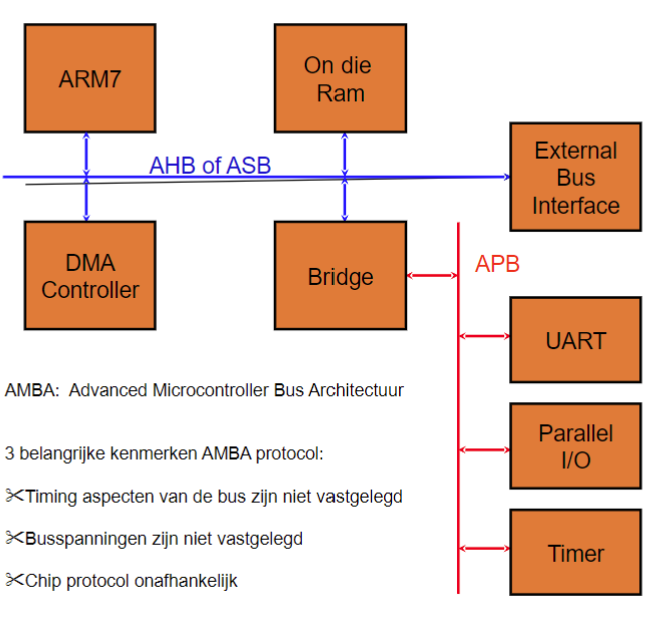
\includegraphics[scale=0.7]{amba.png}
    \end{figure}

\vspace{1cm}

Bus conclusie:\\
AHB gebruiken we als systeembus wanneer een hoge bandbreedte vereist is tussen de macrocellen en de arm processor.\\
ASB is de systeembus voor de midrange toepassingen of de oude arm processors.\\
APB is een aparte bus die men gebruikt als interface naar peripherals met een lage bandbreedte welke geen gebruik maken van pipelining





    \subsection{les 4}
    \input{Laagfrequent/Les 4}

\end{document}
